%Notes by Harsh Mistry 
%CS 349
%Based on Template From  https://www.cs.cmu.edu/~ggordon/10725-F12/template.tex

\documentclass[twoside]{article}
\setlength{\oddsidemargin}{0.25 in}
\setlength{\evensidemargin}{-0.25 in}
\setlength{\topmargin}{-0.6 in}
\setlength{\textwidth}{6.5 in}
\setlength{\textheight}{8.5 in}
\setlength{\headsep}{0.75 in}
\setlength{\parindent}{0 in}
\setlength{\parskip}{0.1 in}
\usepackage{amsmath,amsfonts,graphicx}
\newcounter{lecnum}
\renewcommand{\thepage}{\thelecnum-\arabic{page}}
\renewcommand{\thesection}{\thelecnum.\arabic{section}}
\renewcommand{\theequation}{\thelecnum.\arabic{equation}}
\renewcommand{\thefigure}{\thelecnum.\arabic{figure}}
\renewcommand{\thetable}{\thelecnum.\arabic{table}}
\newcommand{\lecture}[4]{
   \pagestyle{myheadings}
   \thispagestyle{plain}
   \newpage
   \setcounter{lecnum}{#1}
   \setcounter{page}{1}
   
   
%Info Box 
   \begin{center}
   \framebox{
      \vbox{\vspace{2mm}
    \hbox to 6.28in { {\bf CS 349 - User Interfaces
	\hfill Winter 2018} }
       \vspace{4mm}
       \hbox to 6.28in { {\Large \hfill Lecture #1: #2  \hfill} }
       \vspace{2mm}
       \hbox to 6.28in { {\it Lecturer: #3 \hfill Notes By: #4} }
      \vspace{2mm}}
   }
   \end{center}
   
   \markboth{Lecture #1: #2}{Lecture #1: #2}



 
}

\renewcommand{\cite}[1]{[#1]}
\def\beginrefs{\begin{list}%
        {[\arabic{equation}]}{\usecounter{equation}
         \setlength{\leftmargin}{2.0truecm}\setlength{\labelsep}{0.4truecm}%
         \setlength{\labelwidth}{1.6truecm}}}
\def\endrefs{\end{list}}
\def\bibentry#1{\item[\hbox{[#1]}]}

\newcommand{\fig}[3]{
			\vspace{#2}
			\begin{center}
			Figure \thelecnum.#1:~#3
			\end{center}
	}
	
\graphicspath{ {images/} }

\newtheorem{theorem}{Theorem}[lecnum]
\newtheorem{lemma}[theorem]{Lemma}
\newtheorem{ex}[theorem]{Example}
\newtheorem{proposition}[theorem]{Proposition}
\newtheorem{claim}[theorem]{Claim}
\newtheorem{corollary}[theorem]{Corollary}
\newtheorem{definition}[theorem]{Definition}
\newenvironment{proof}{{\bf Proof:}}{\hfill\rule{2mm}{2mm}}
\newcommand\E{\mathbb{E}}


%Start of Document 
\begin{document}

\lecture{7}{January 18, 2018}{Keiko Katsuragawa}{Harsh Mistry}

\section{Widgets}

\begin{itemize}
\item Widget is a generic name for parts of an interface that have their own behavior: buttons, drop-down menus, spinners, file dialog boxes, progress bars, sliders, ...
\item widgets also called components, or controls
\item They provide user feedback and capture user input
\item They have a defined appearance
\item They send and receive events 
\end{itemize}

\subsection{Logical Device}
\begin{itemize}
\item A logical device is the essence of what a widget does. Its function
\item E.g logical button device. The function is to generate a pushed event.
\item A widget is a logical device with an appearance. 
\end{itemize}

\subsection{Categorizing and Characterizing Widgets}
\begin{itemize}
\item Logical Device (Button, number, text, choice, etc)
\item Event the widget generates (action, change, etc)
\item Properties to change behaviour and appearance (colour, size, icon, allowable values)
\end{itemize}

\subsection{Simple Widgets}
\begin{center}
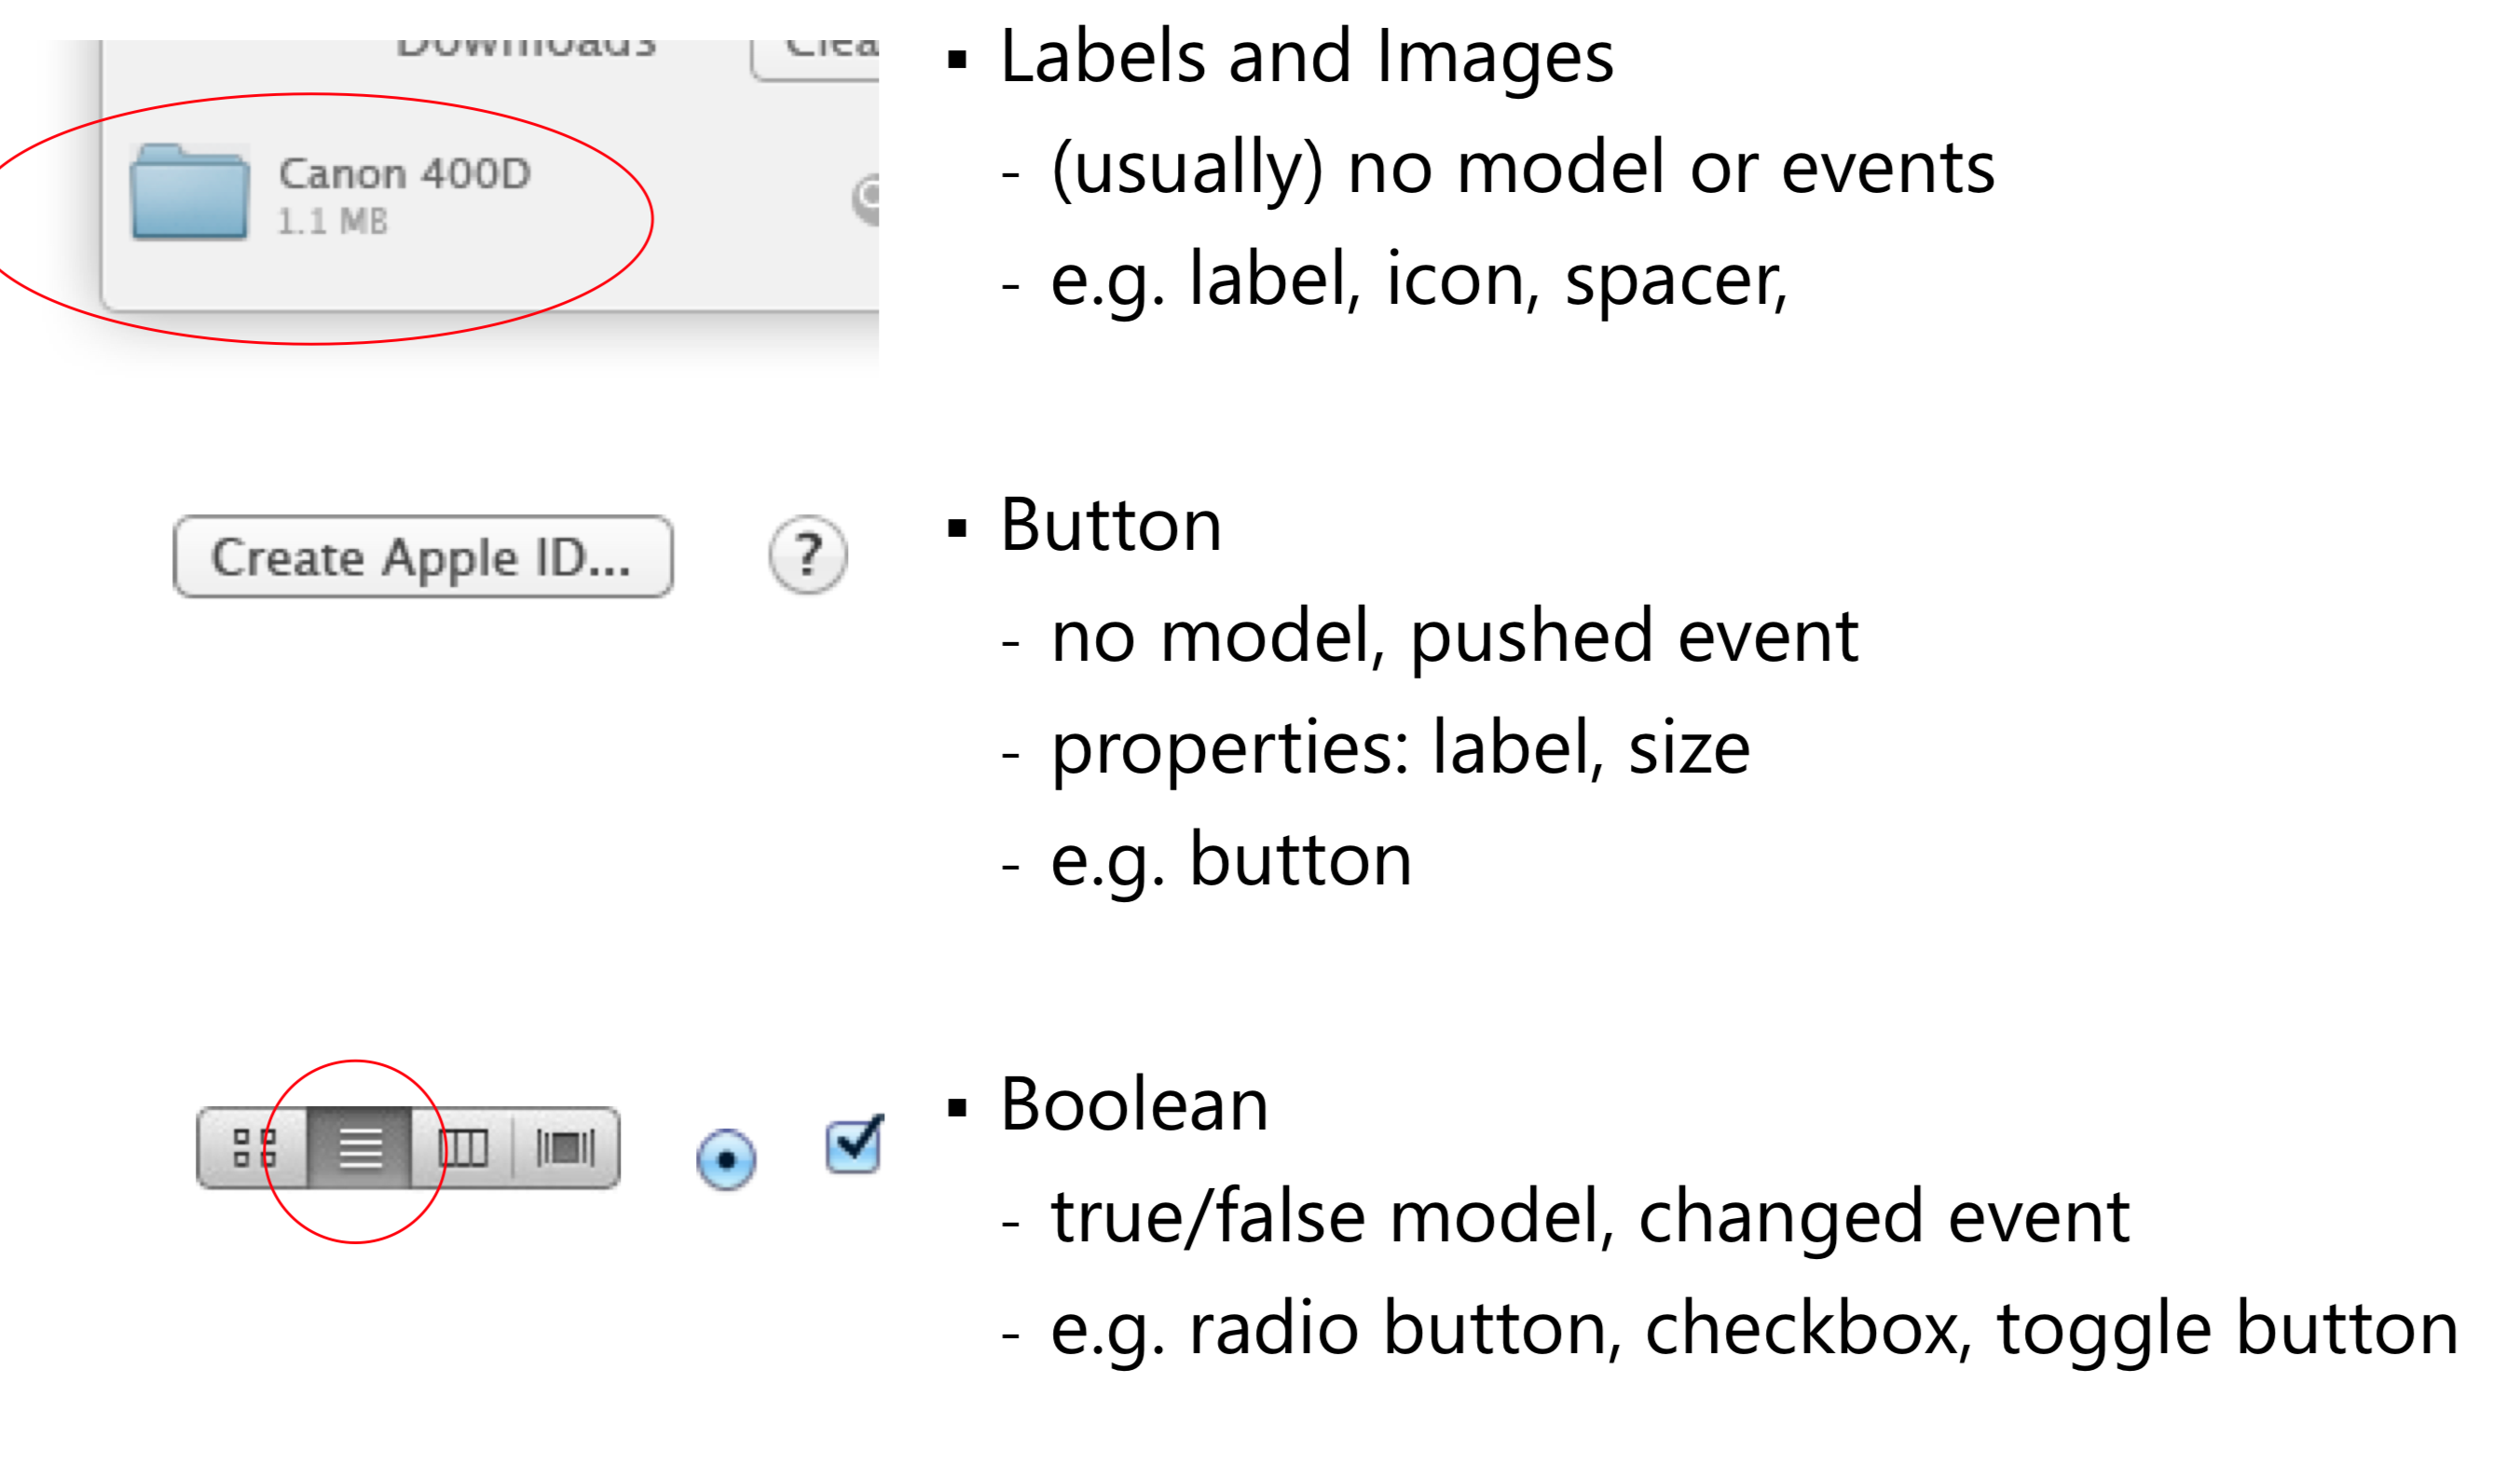
\includegraphics[scale=0.2]{16}\\
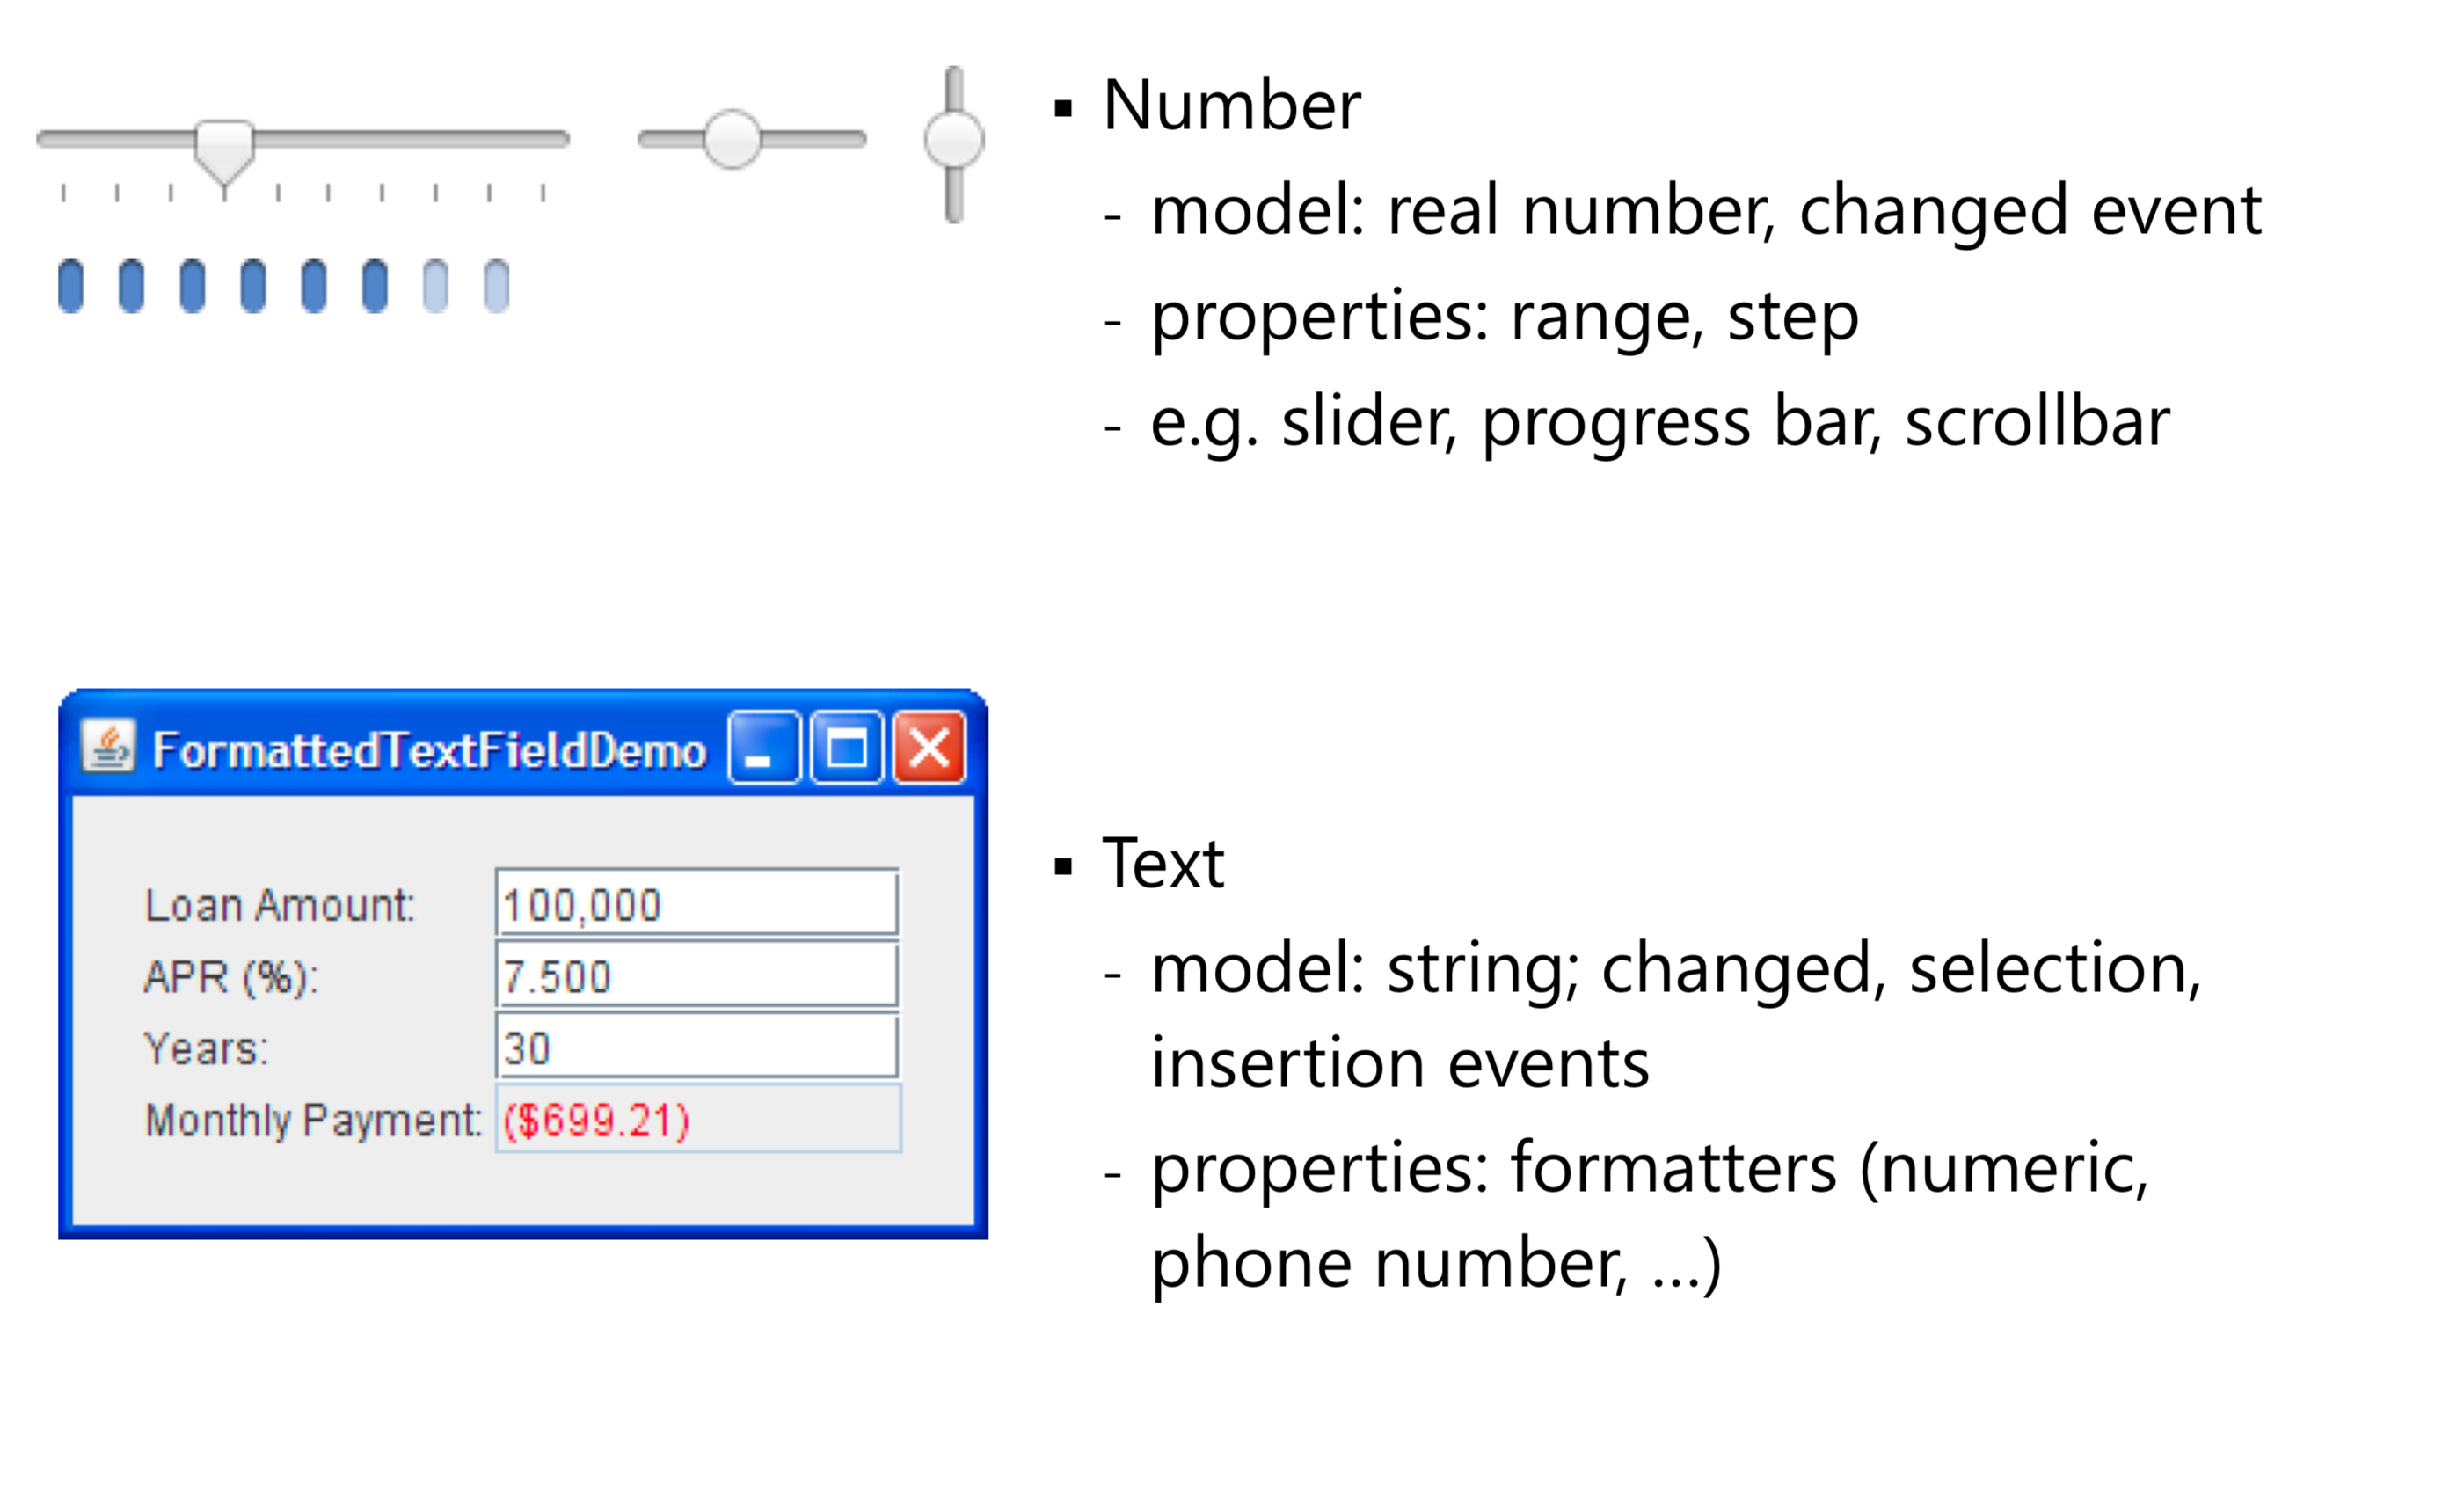
\includegraphics[scale=0.2]{17}\\
\end{center}

\subsection{Container Widgets}
\begin{center}
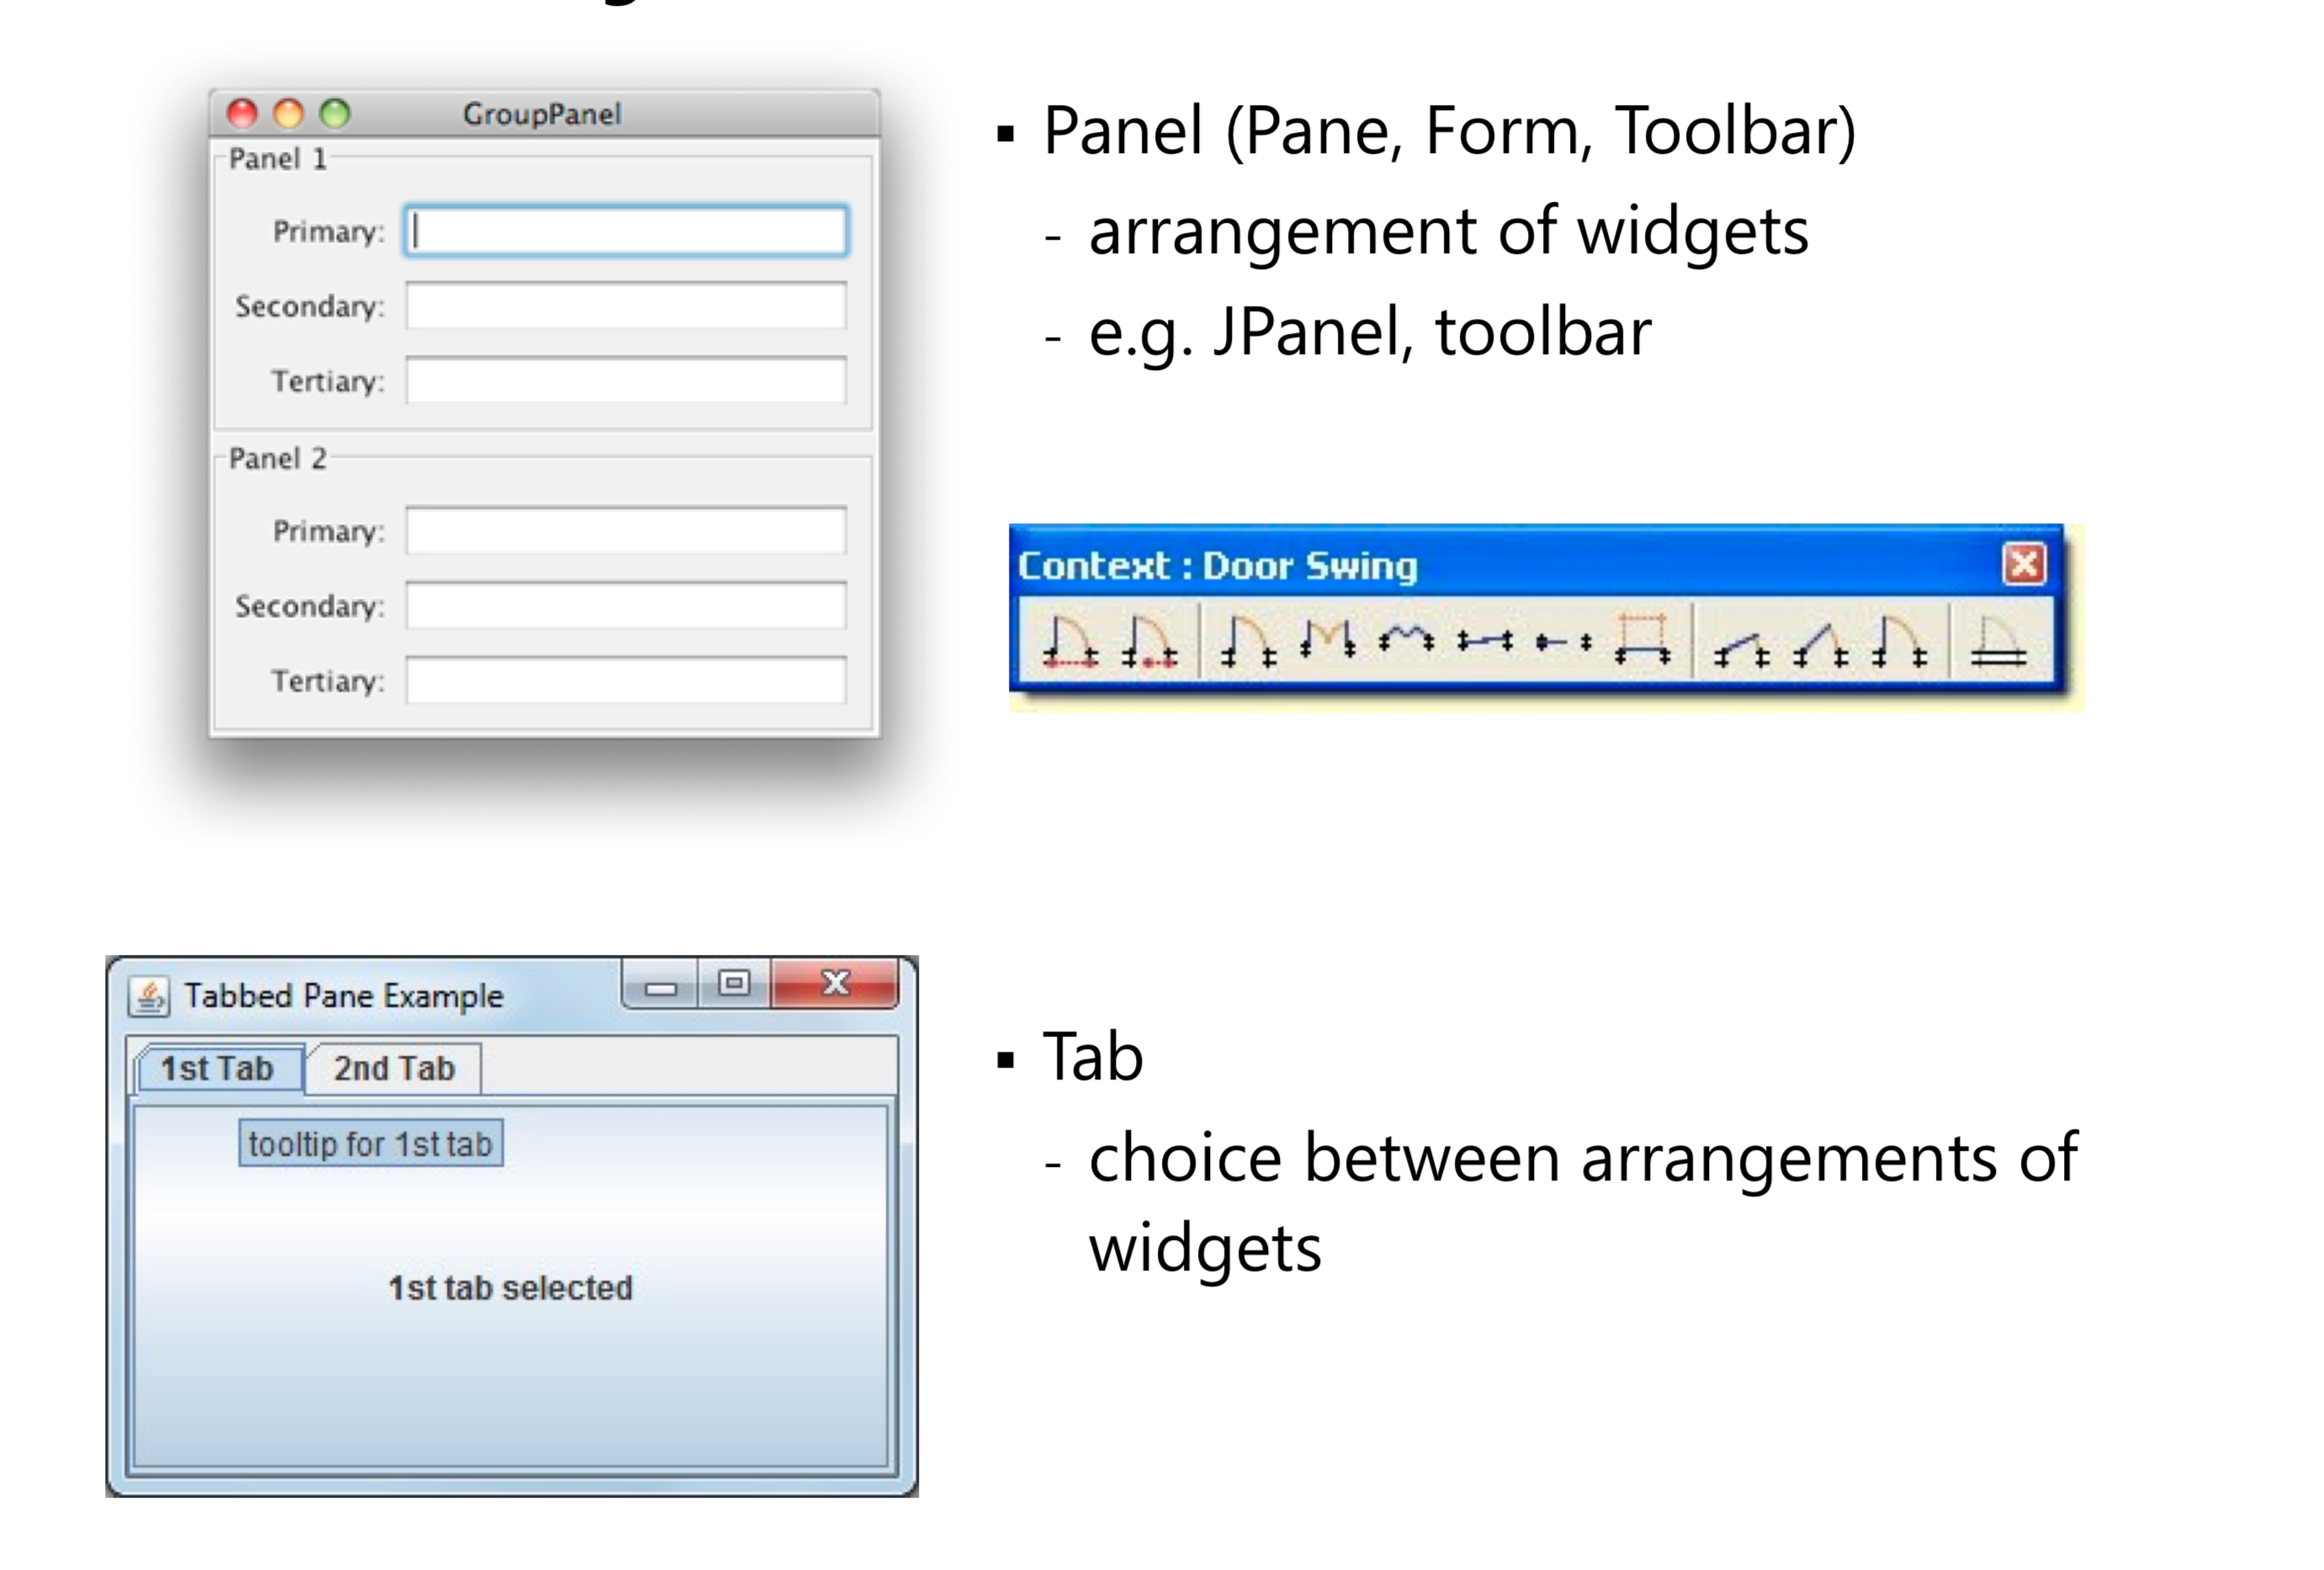
\includegraphics[scale=0.2]{18}\\
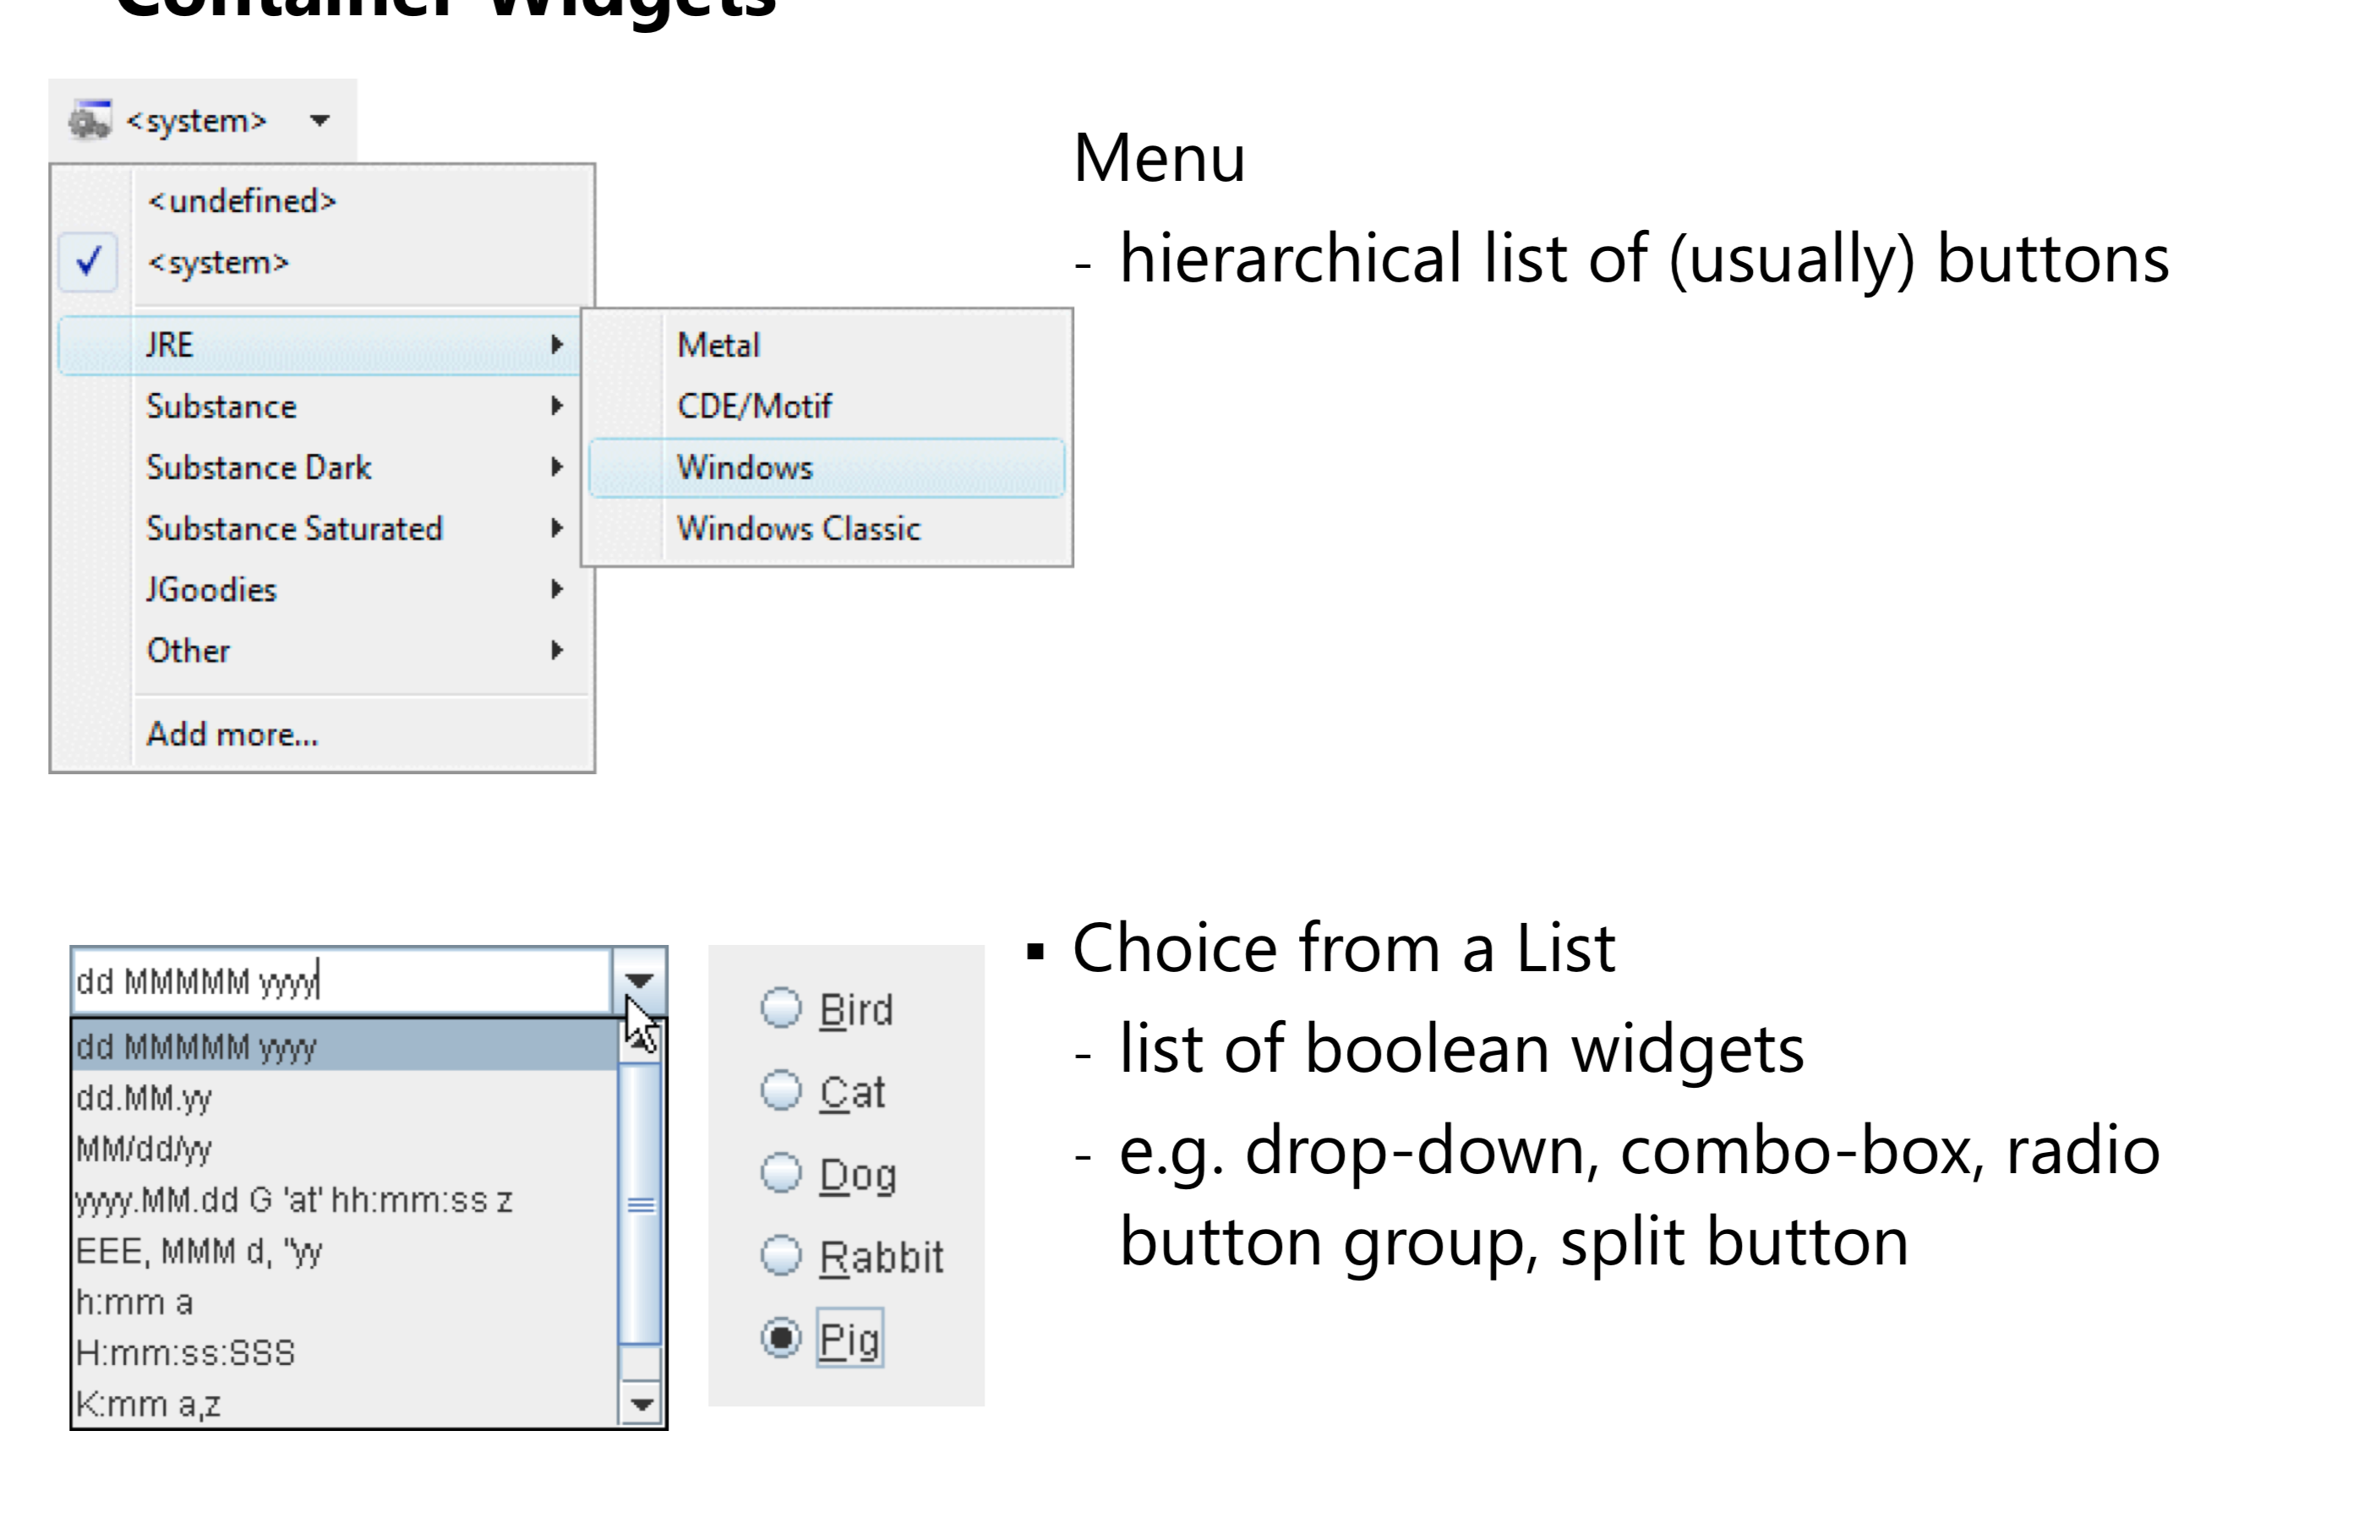
\includegraphics[scale=0.2]{19}\\
\end{center}

\subsection{Special Value Widgets}
\begin{center}
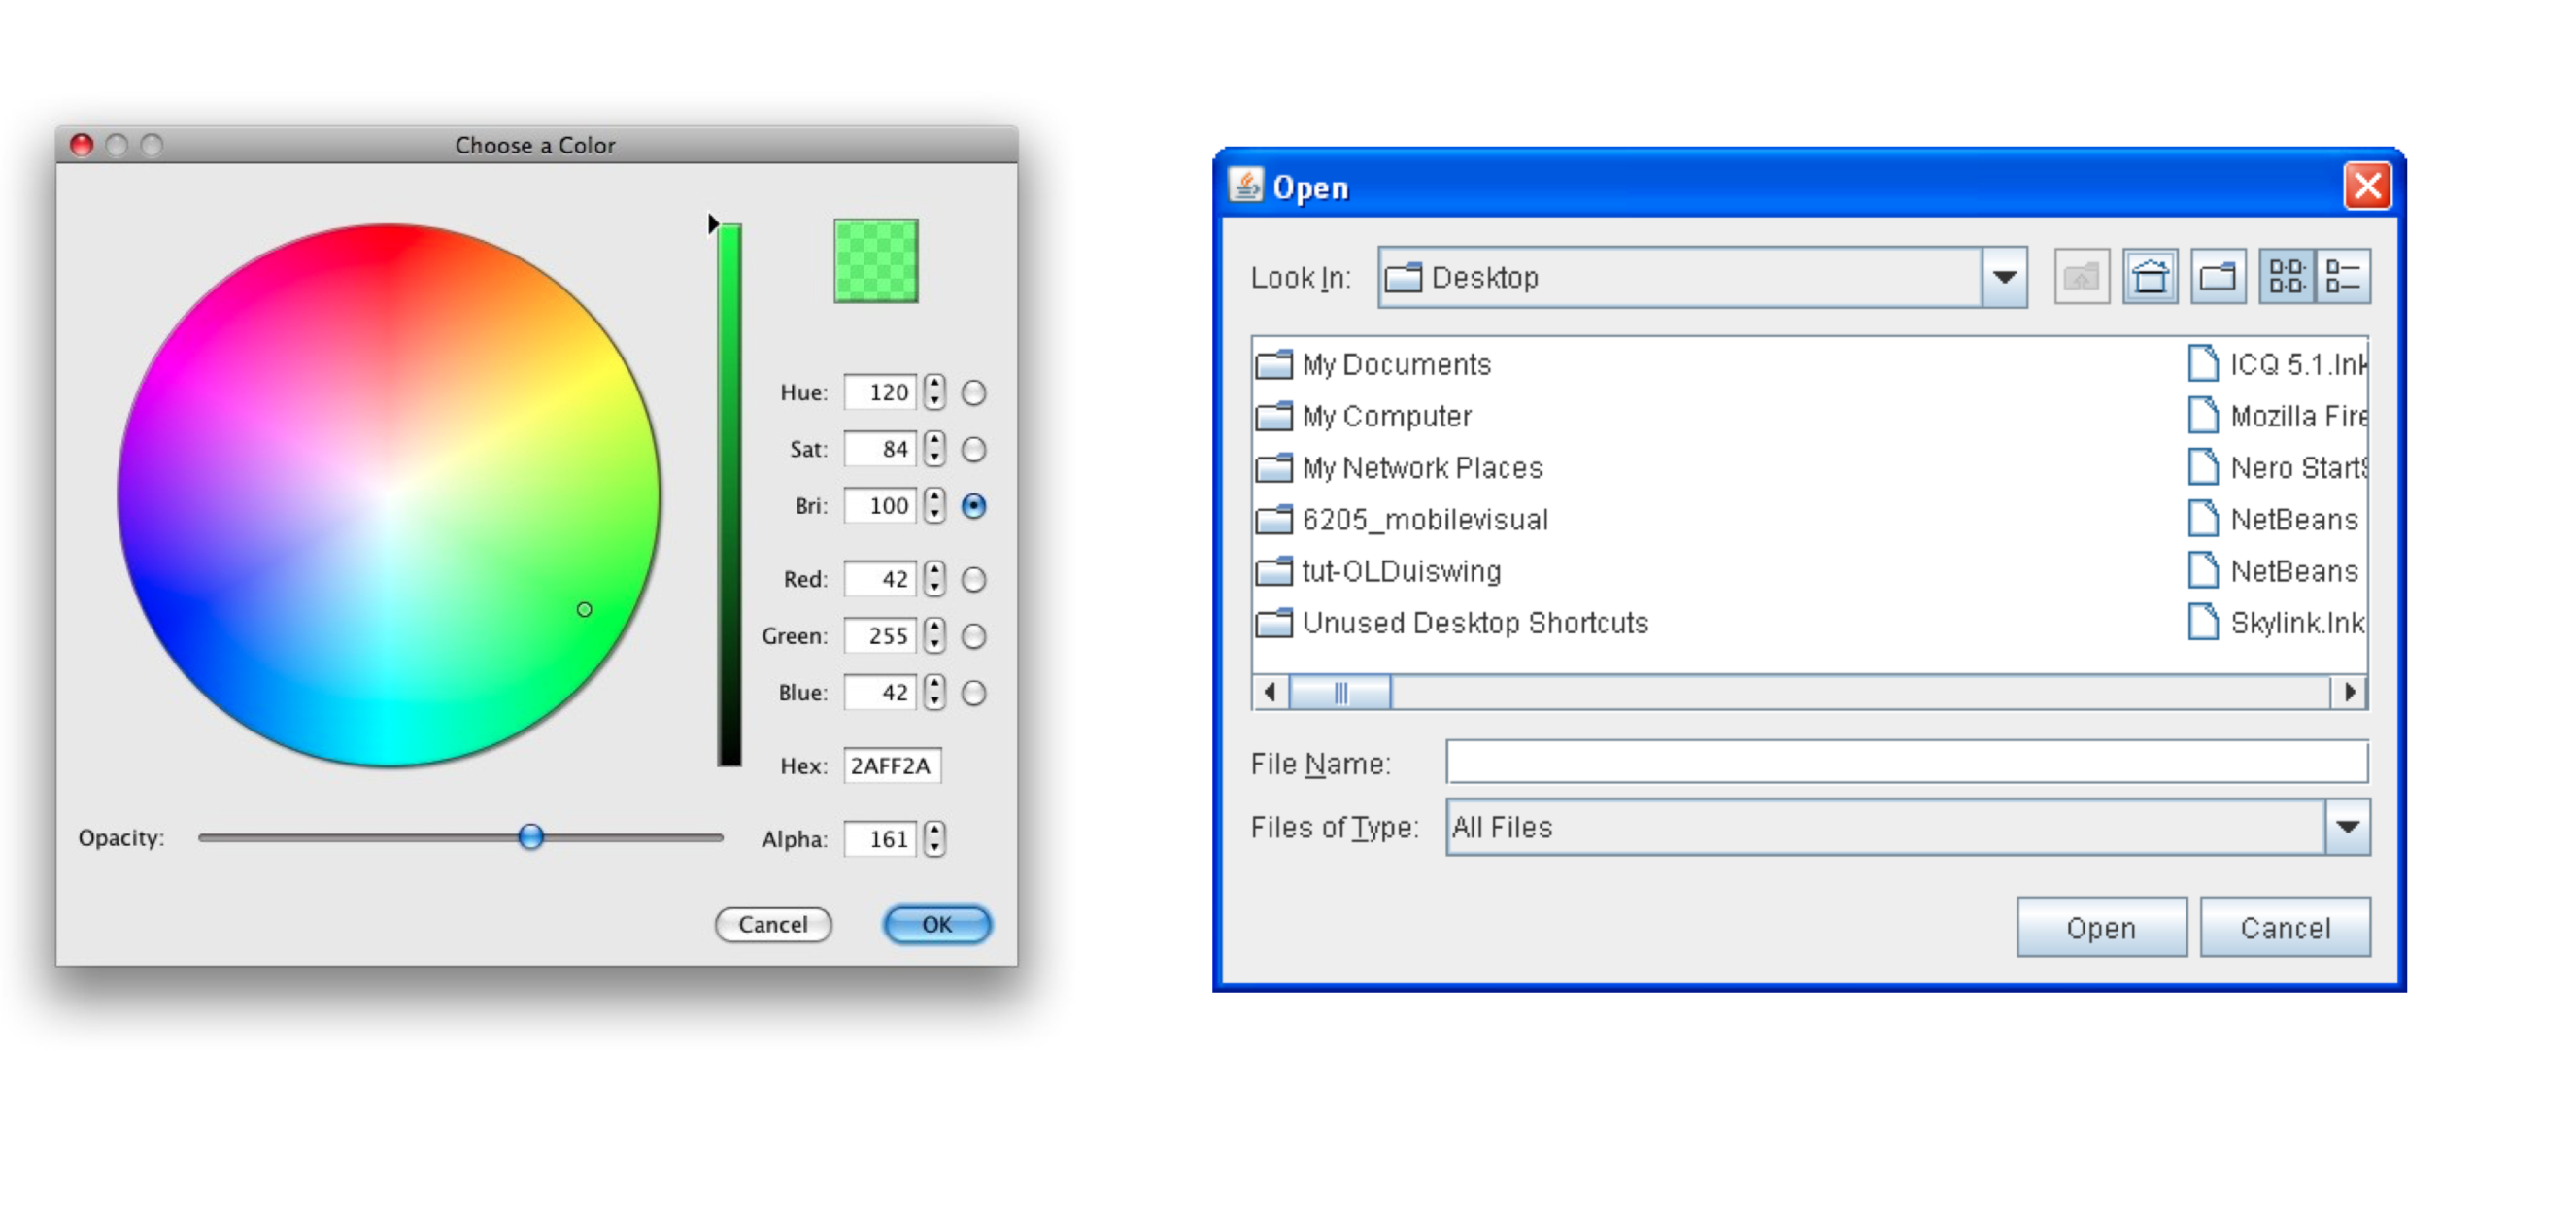
\includegraphics[scale=0.2]{20}
\end{center}

\subsection{Widget toolkits}
\begin{itemize}
\item Also called widget libraries or GUI toolkits or GUI APIs
\item  Software bundled with a window manager, operating system,
development language, hardware platform
\item Defines a set of GUI components for programmers
\item Examples: buttons, drop-down menus, sliders, progress bars, lists,
scrollbars, tab panes, file selection dialogs, etc.
\item Programmers access these GUI components via an application programming interface (API)
\end{itemize}

\subsection{Event-driven programming}
\begin{itemize}
\item Widget toolkits use event-driven programming model
\item Reactive systems 
\begin{itemize}
\item User Action \(\rightarrow\) program response
\item Most of the time the program sits around doing nothing
\end{itemize}
\item Widget toolkit supports a mechanism for mapping user action on widget to appropriate application code to handle that action
\end{itemize}

\begin{center}
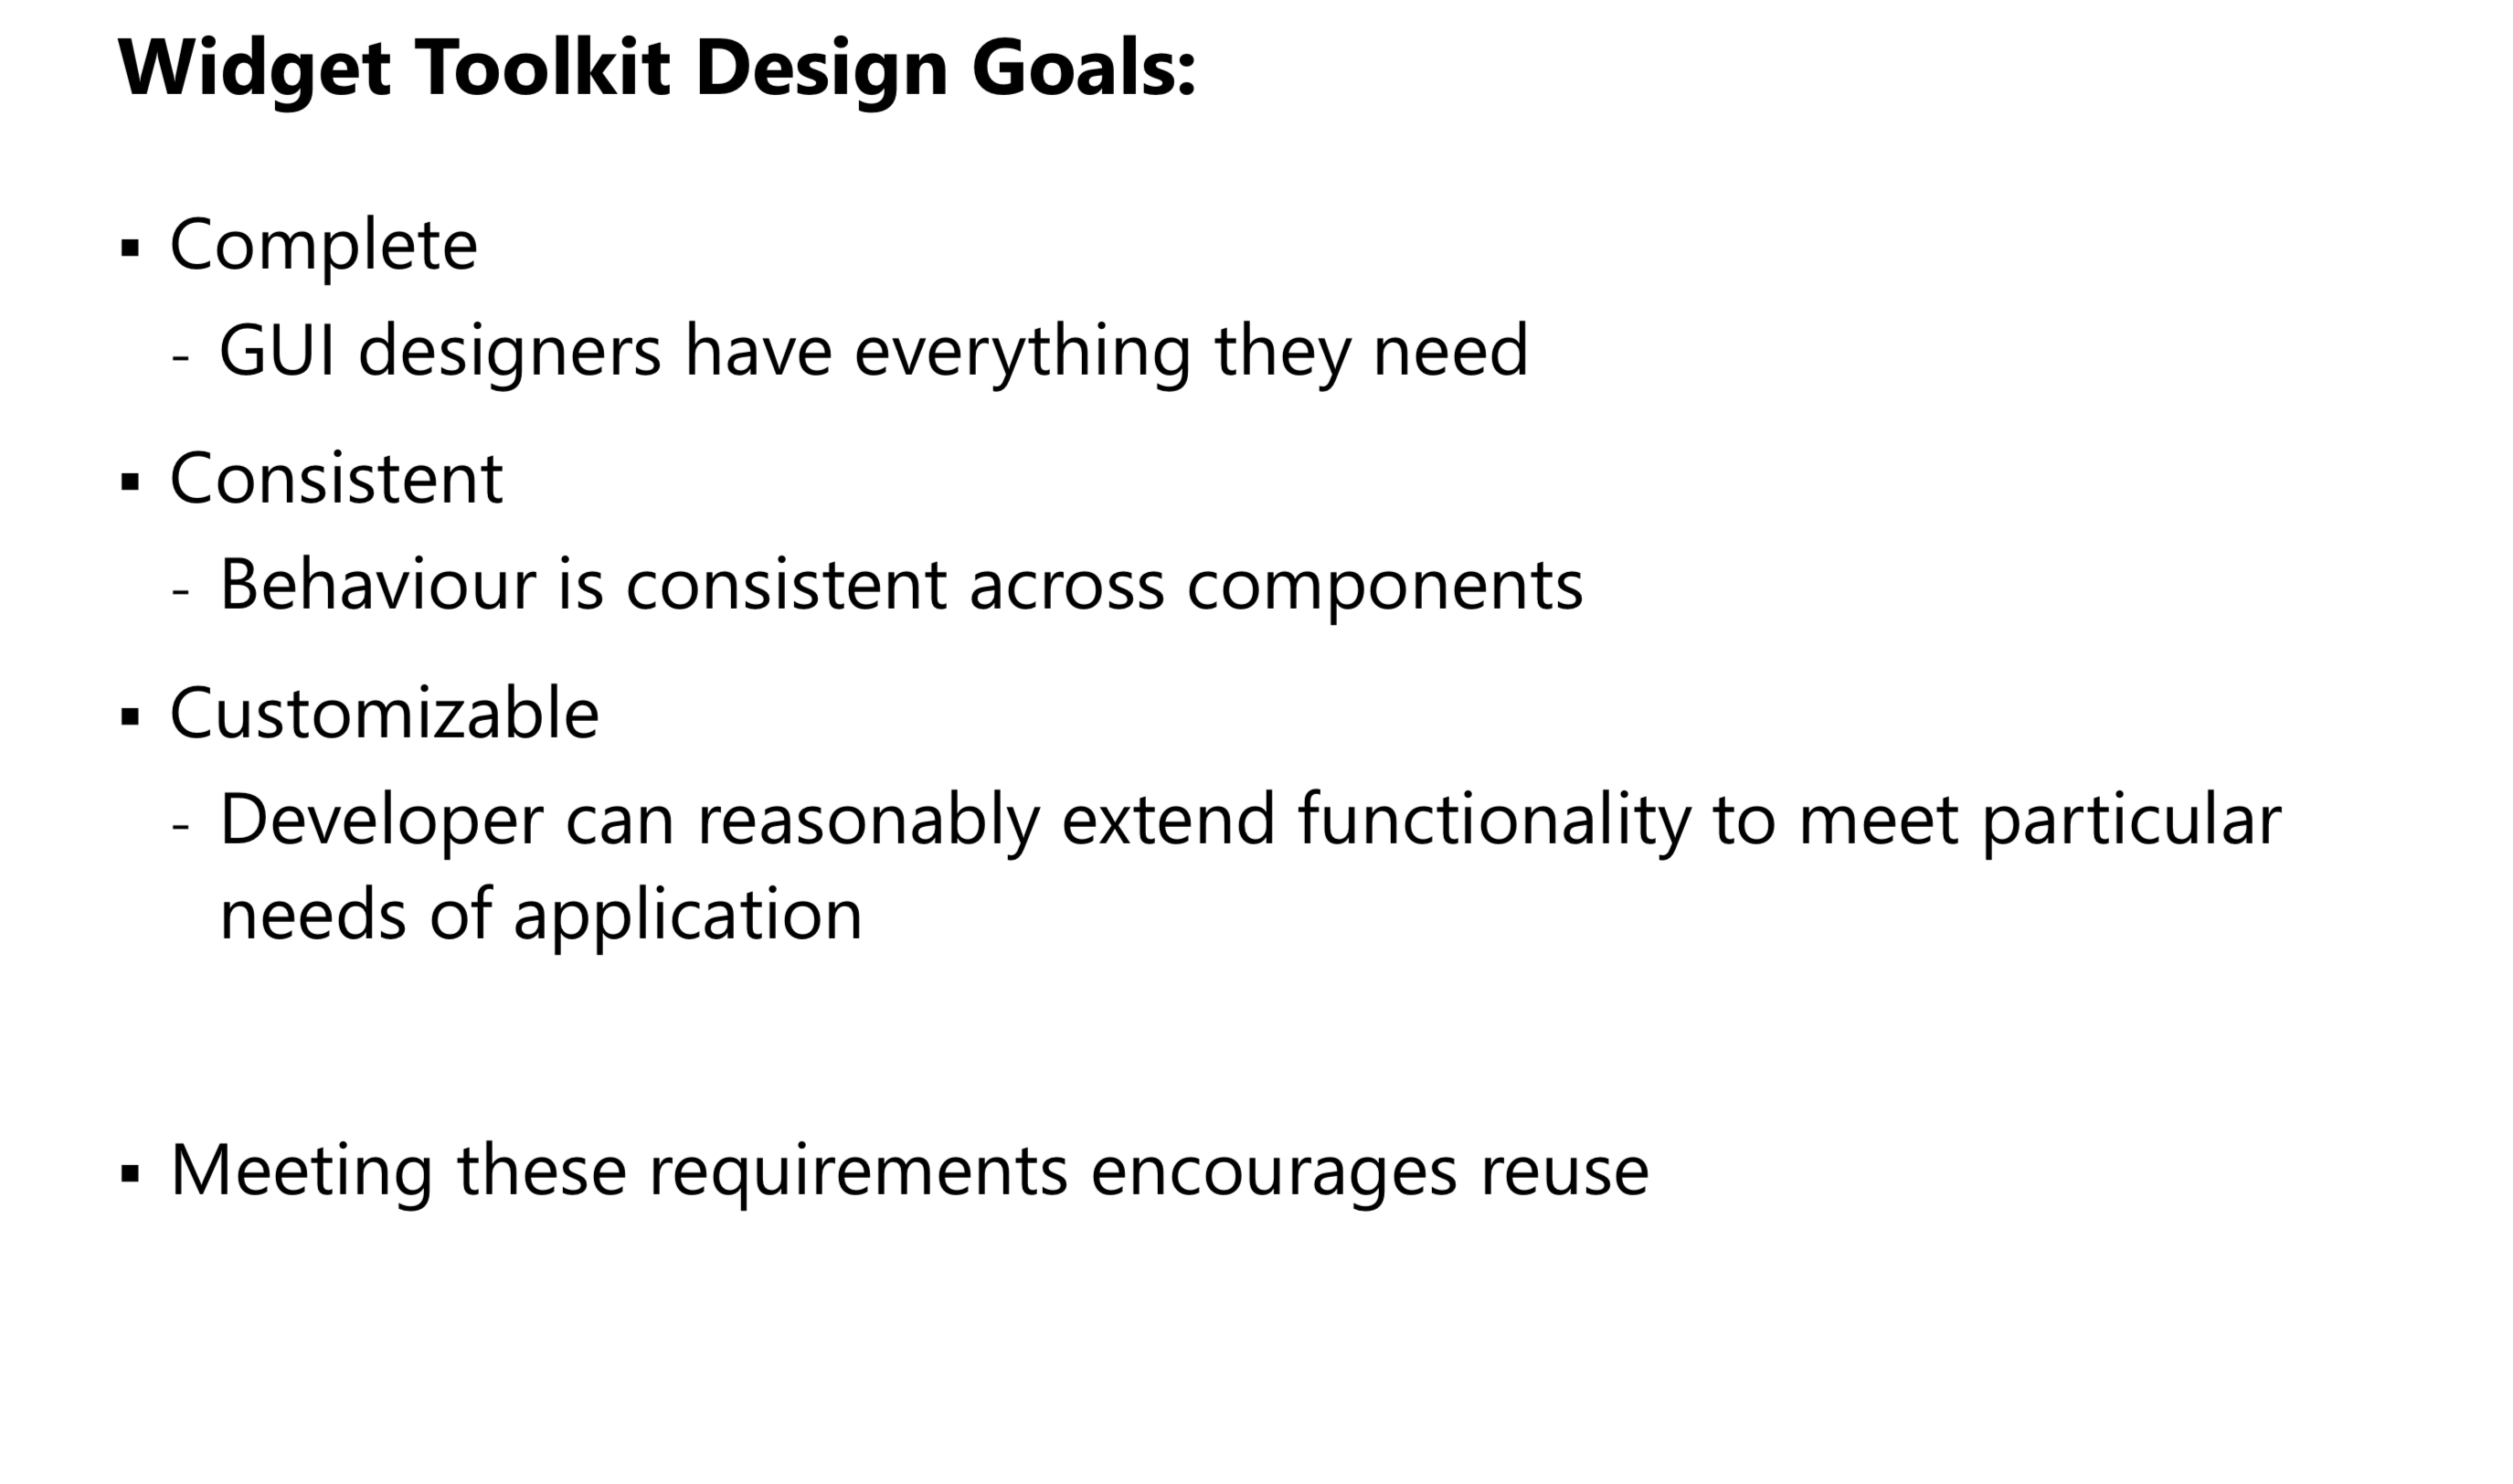
\includegraphics[scale=0.2]{21}
\end{center}

\subsection{Completeness}
\begin{itemize}
\item All you really need are
\begin{itemize}
\item Button 
\item Slider
\item Pulldown menu
\item Check box
\item Radio button 
\item Text field
\end{itemize}
\end{itemize}

\section{Heavyweight Widgets}
\begin{center}
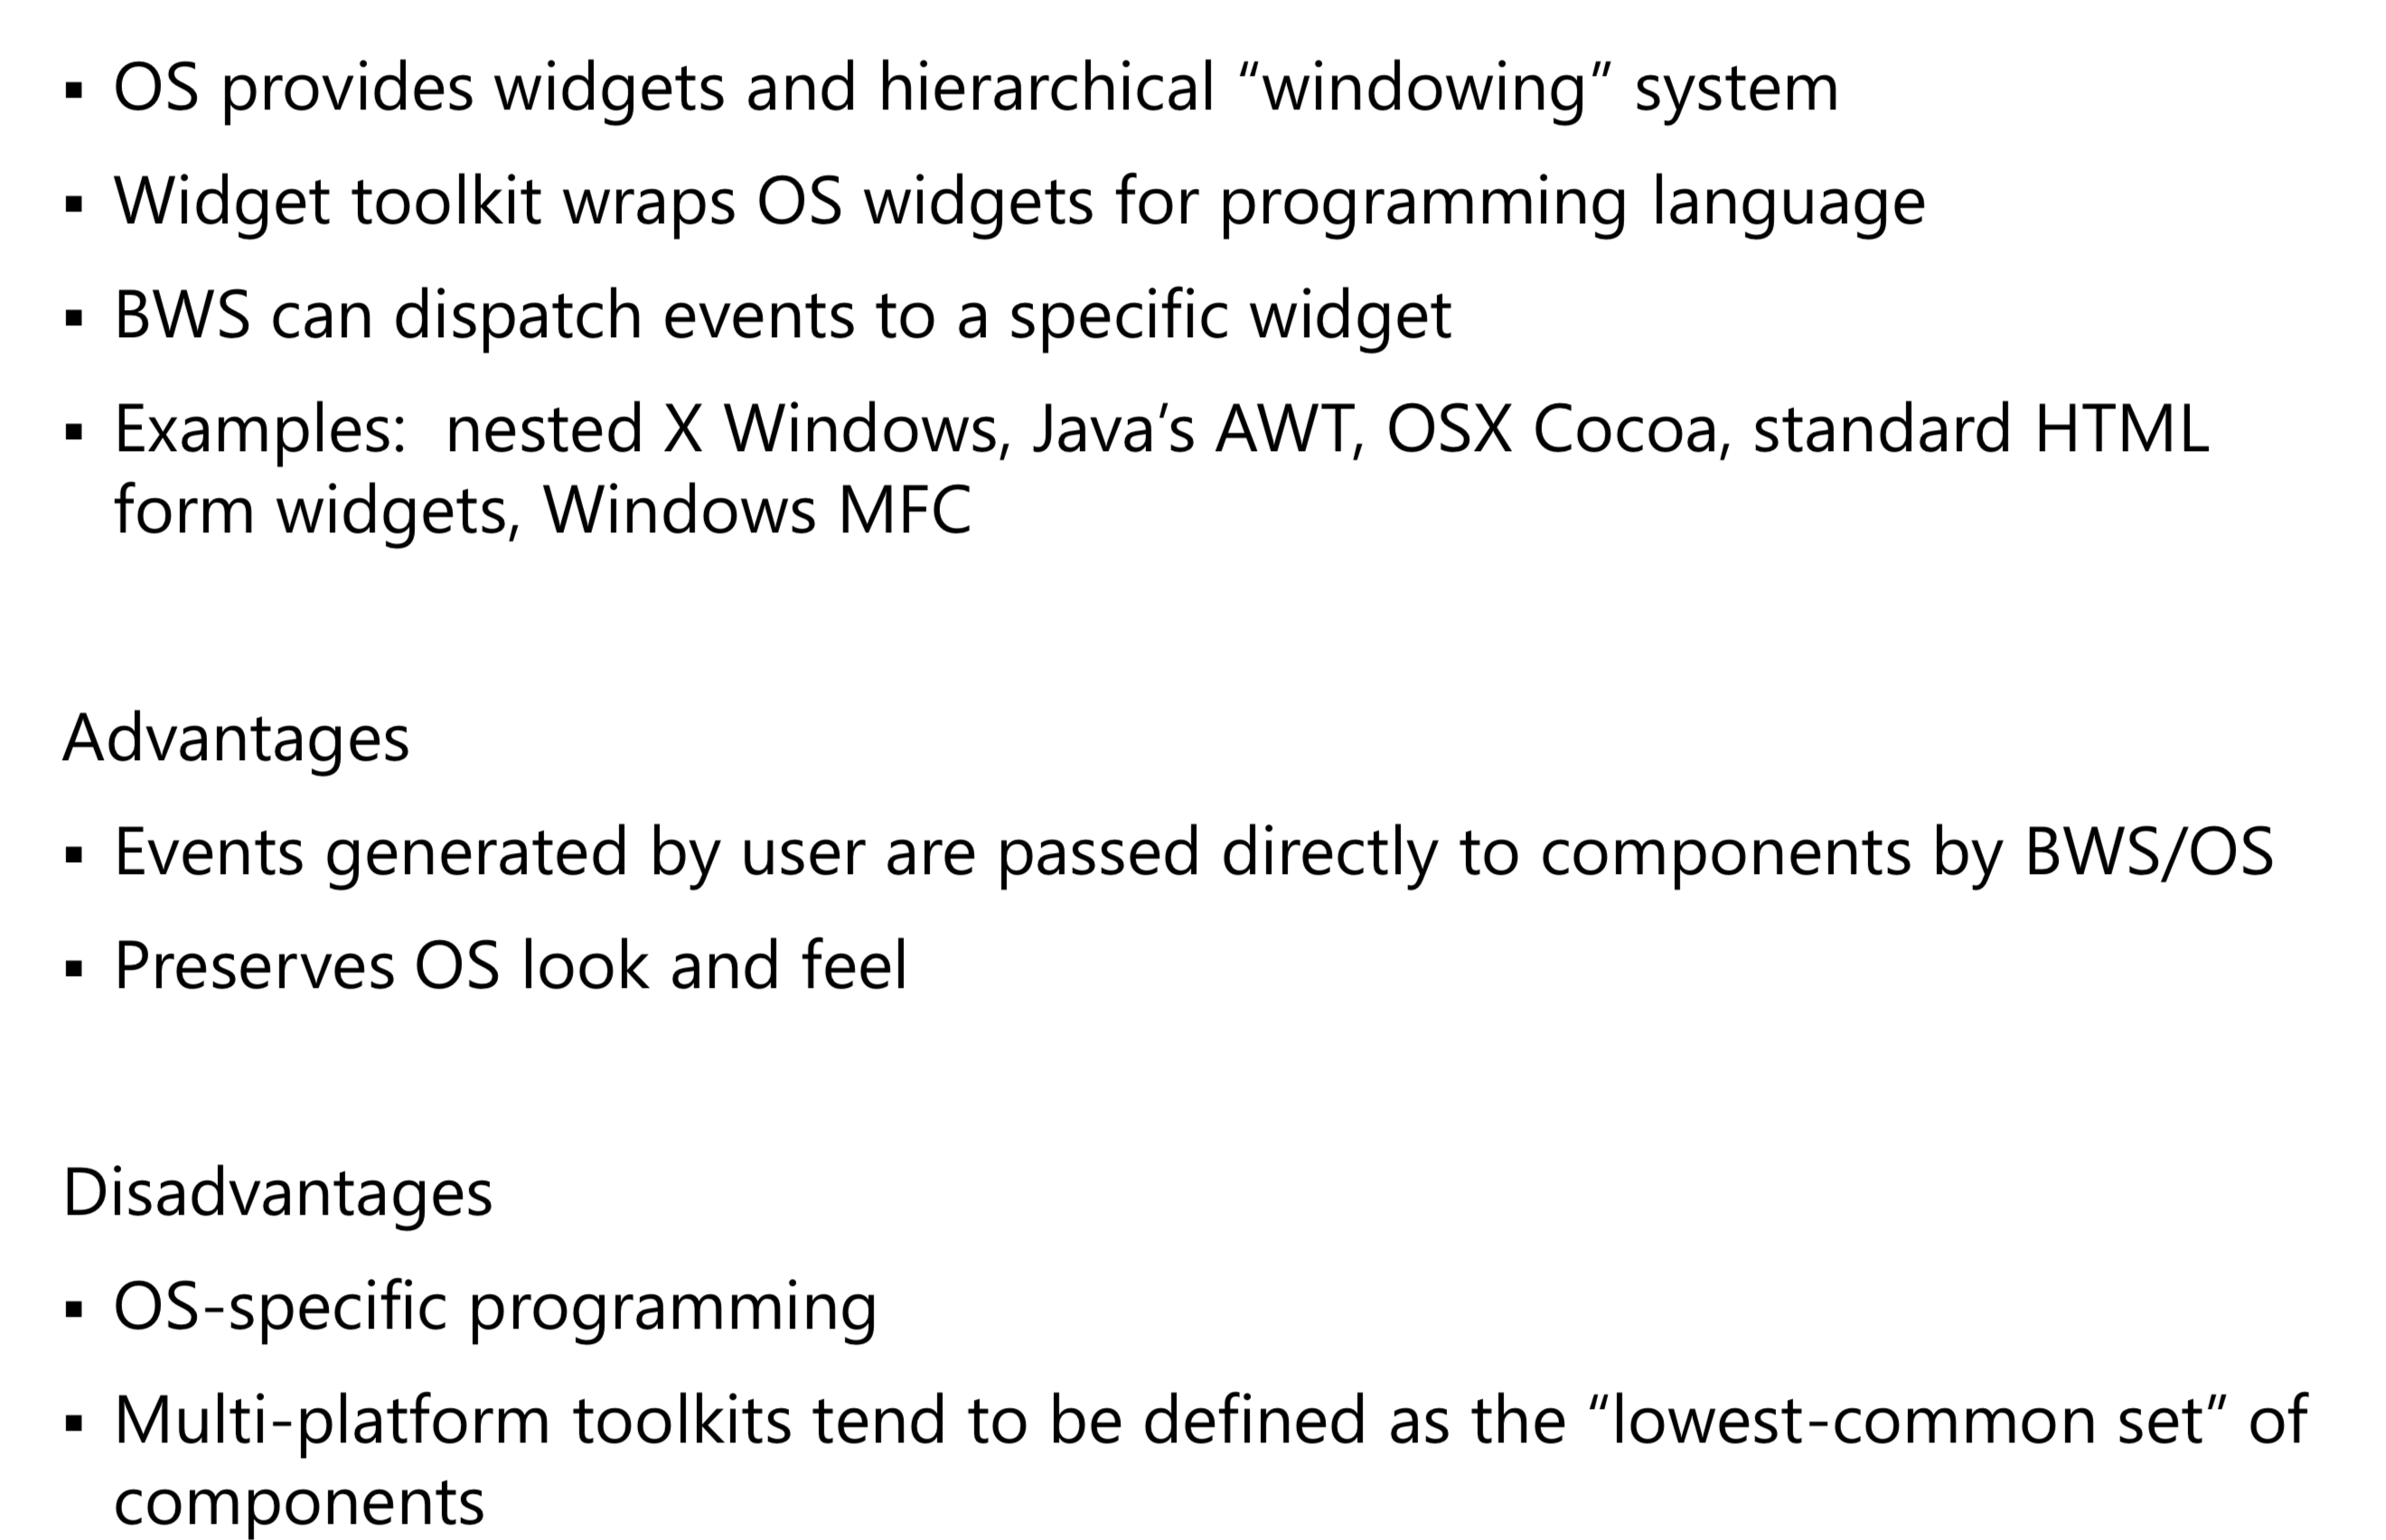
\includegraphics[scale=0.2]{22}\end{center}

\section{Lightweight Widgets}
\begin{center}
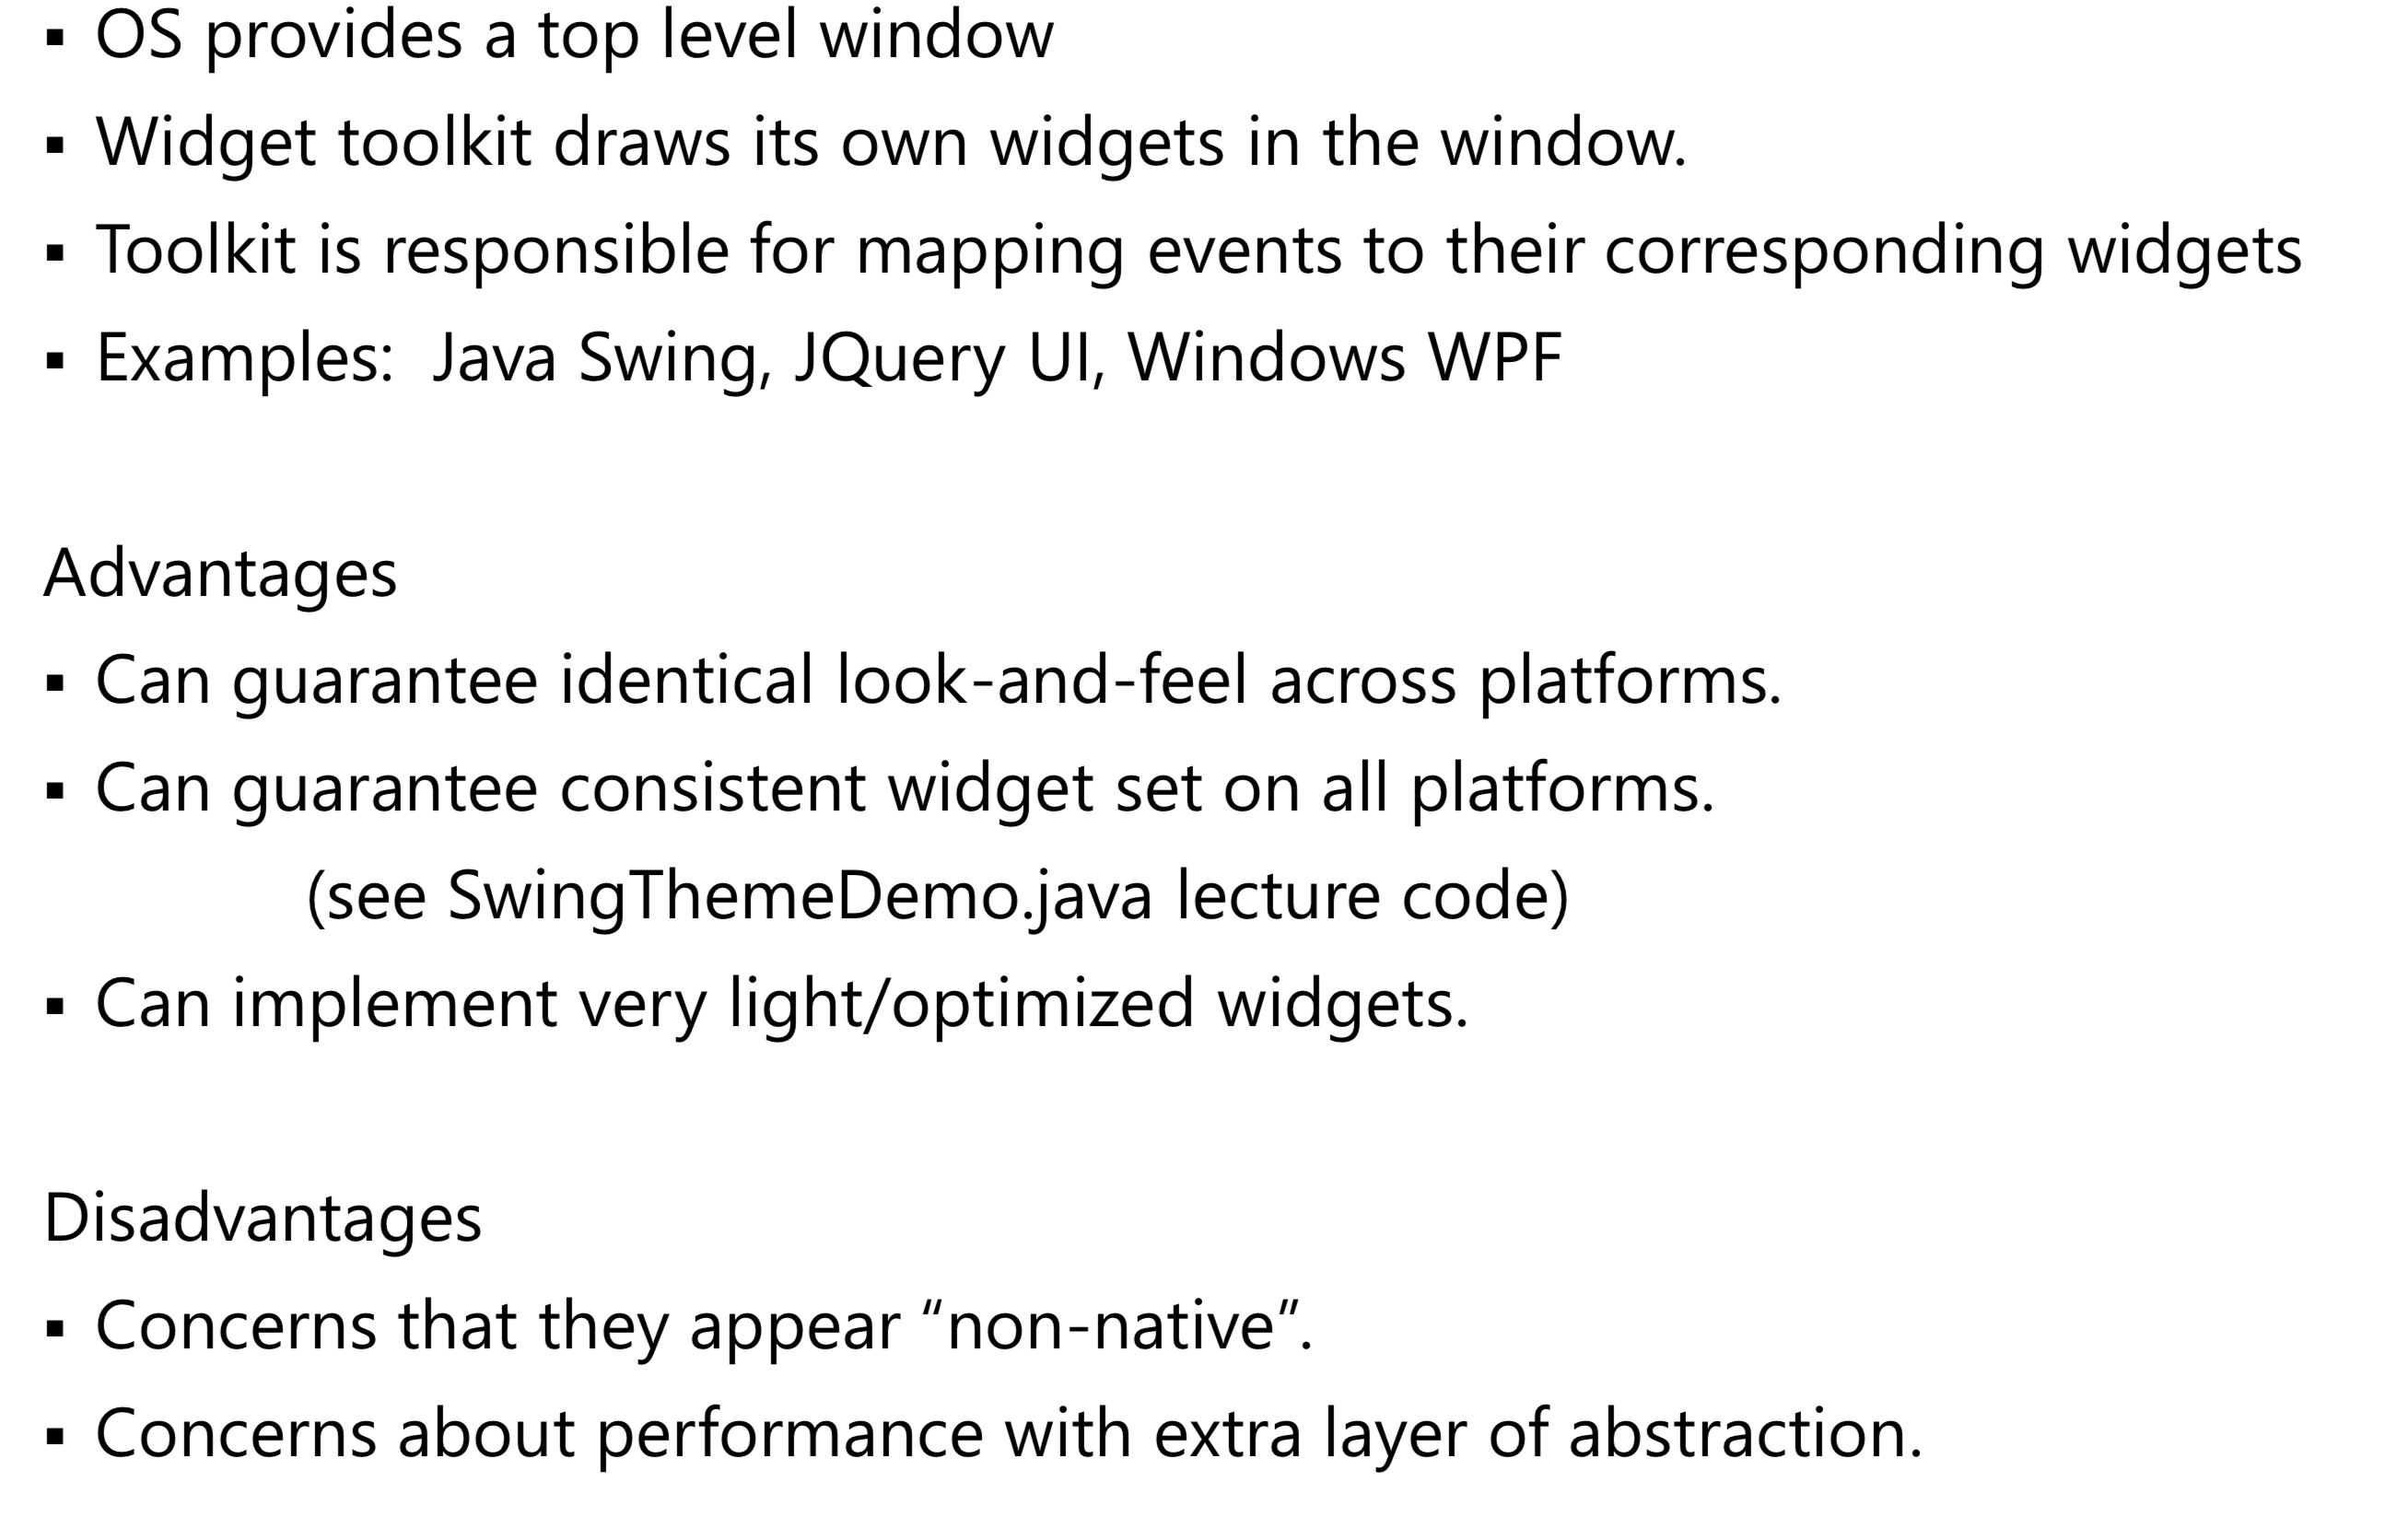
\includegraphics[scale=0.2]{23}\end{center}

\end{document}





